\documentclass[a4paper,11pt]{kth-mag}
\usepackage[T1]{fontenc}
\usepackage{textcomp}
\usepackage{lmodern}
\usepackage[latin1]{inputenc}
\usepackage[swedish,english]{babel}
\usepackage{modifications}
\usepackage{hyperref}
\usepackage{graphicx}



\newcommand{\Cpp}{\texttt{C++}}
\newcommand{\Gcc}{\texttt{gcc}}
\newcommand{\Gtkmm}{\texttt{gtkmm}}
\newcommand{\Gtk}{\texttt{GTK+}}


\title{SimpleGraphPlotter v1.6}

\subtitle{}
\foreigntitle{}
\author{Jim Holmstr\"{o}m\\\href{mailto:jimho@kth.se}{jimho@kth.se}}
\date{\today}
\blurb{}

%\trita{TRITA xxx yyyy-nn}
\trita{}
\begin{document}
\frontmatter
\pagestyle{empty}
\removepagenumbers
\maketitle
\selectlanguage{english}
\tableofcontents*
\mainmatter
\pagestyle{newchap}

\chapter{Introduction}
In the following part firstly the problem will be explained and secondly the requirements for a basic plotter will be enlisted.
A plotter is a program that can plot functions from strings which defines the functions by ordinary math syntax. 
This project uses \Cpp~ programming language and a the 
\Gtkmm\footnote{Documentation, binaries and source can be found at: \href{http://www.gtkmm.org}{www.gtkmm.org}} wrapper for the 
\Gtk\footnote{Documentation, binaries and source can be found at: \href{http://www.gtk.org}{www.gtk.org}} toolkit to generate the graphical user interface. 
It is compiled with the \texttt{GNU} \Gcc compiler.

\section{Requirements}
A few basic things is needed to have a functioning math plotter:
\begin{enumerate}
    \item Define a function given ordinary math syntax.
    \item Parse the inputed function and plot it accordingly.
    \item Add/Remove functions from plotarea.
    \item Plotarea should be scrollable both vertical and horizontal.
    \item Range should be fixed to the unit-cube.\footnote{This restriction will be handled in section \ref{sec:scope}}
    \item Display axis of the plot.
    \item Parser must be properly tested.
\end{enumerate}

\section{Scope}
\label{sec:scope}
The amount of functionallity that is possible to put in a system like this is almost endless so a few delimitations has to be made in order to complete the project.
The currently biggest restriction to the plotter is the lack of ability to zoom or change the range from the unit-cube.
No support for parametric nor complex functions.
\footnote{Since no native support in \Cpp~ for complex numbers which means all the basic math functions would have to be rewritten in order for this to work.}

\chapter{Structure}
An basic overview can be seen in figure \ref{fig:UML}
\section{UML}
\begin{figure}[ht]
    \begin{center}
        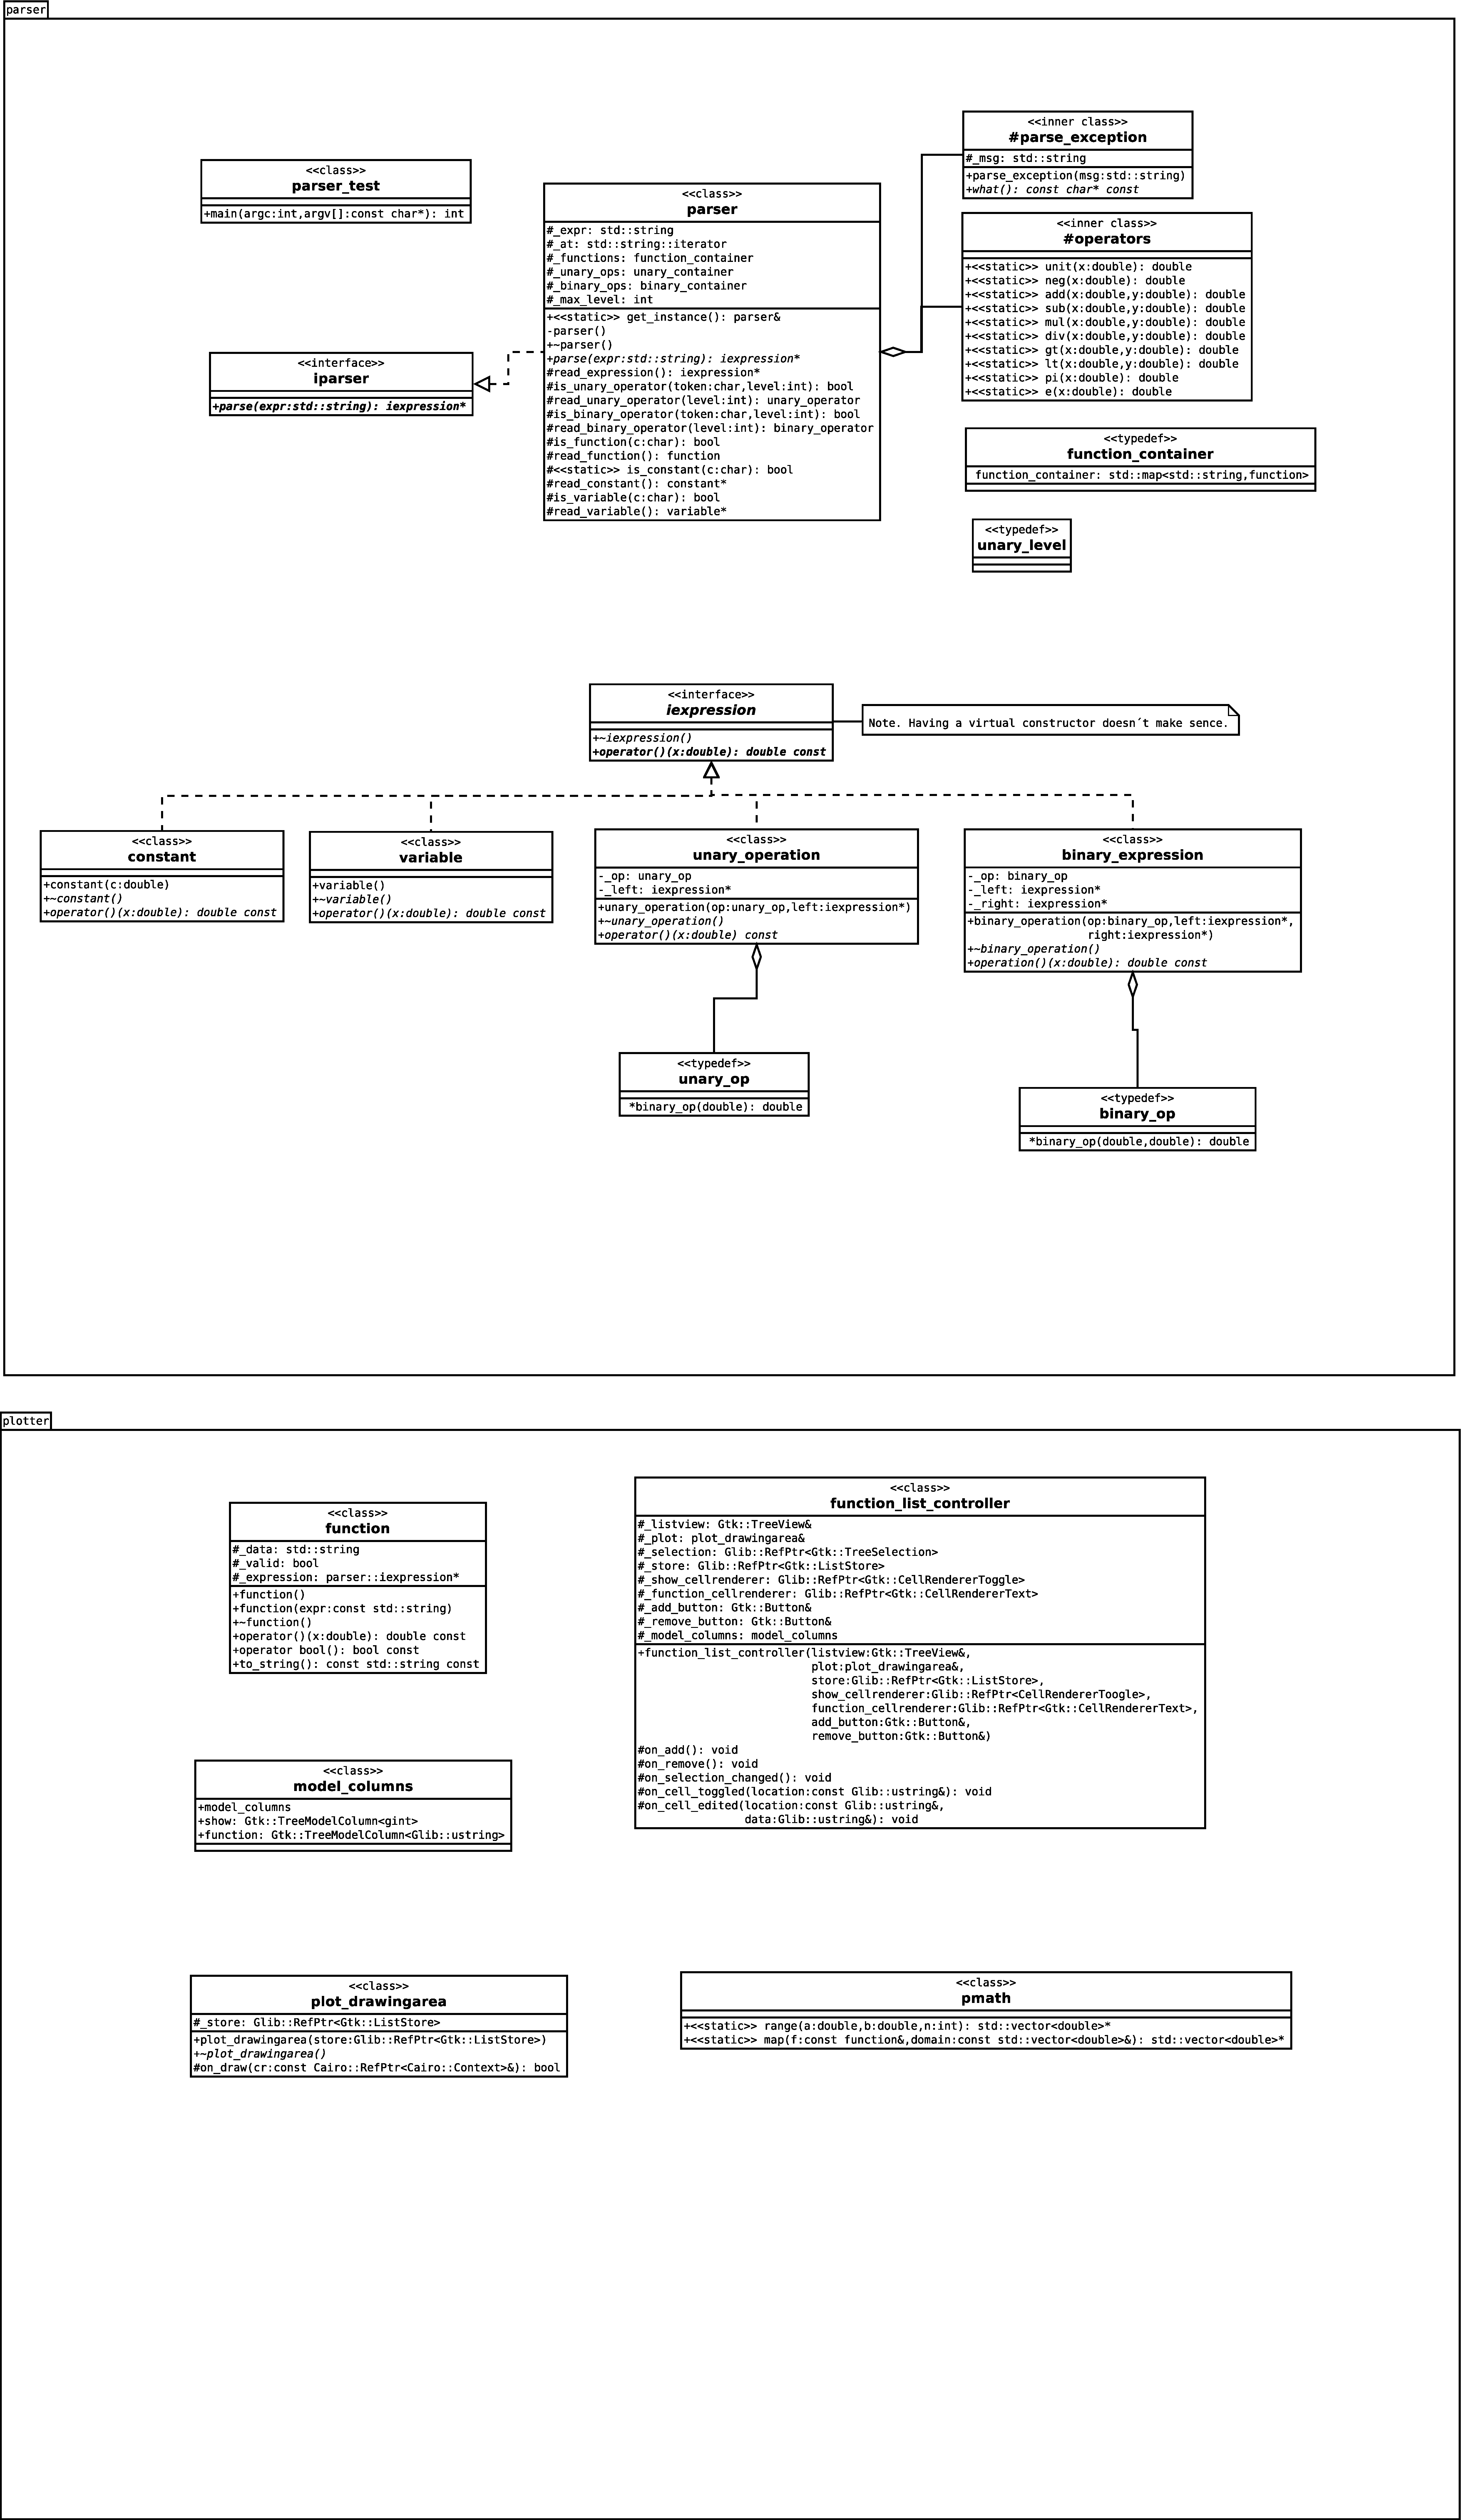
\includegraphics[width=\textwidth]{uml.pdf}
        \caption{\small{An UML showing the structure and the enclosure.}}\label{fig:UML}
    \end{center}
\end{figure}




\chapter{Results and Discussion}
* Problems with the unofficial c++ wrapper gtkmm, only used it to avoid missing out 
*


\end{document}
